\chapter{Results and Discussion}
In this chapter, we show results of applying the regression algorithms on our dataset for estimating DHI (Diffuse Horizontal Irradiance) from sky images. As the metric for comparison between methods, Root Mean Square Error(RMSE) is used. We will also discuss where the algorithms perform poorly by showing cases.

\section{Feature Selection}
Since the correlation of each feature element to DHI is not strong enough, for we need to do a feature selection in order to select the most relevant features and discard the ones that are not helpful enough. For that purpose, we use a Forward-Selection algorithm for each method. This approach assumes an empty feature vector initially, and at every iteration evaluate the error of estimation after adding each one of the available feature elements to current feature set. The feature set with least error will be chosen and removed from available feature elements. However, the difference of last error and current error has to be more than a threshold for adding that feature elements. This helps to exclude random improvements caused by features and don't add them to final feature set. This threshold has been set empirically to 0.7 in RMSE -60\% of inverse of chi-square cumulative distribution function for 1 degree of freedom. 
\newline
To verify the advantage of using image features along non-image features in the feature vector, we evaluate these two cases separately by each regression method. The non-image feature set consists of [clear-sky-DHI, sun-zenith]. The full feature vector includes: [sun-state, saturation factor, cloud coverage of region 1, region 2, region 3, region 4, clear-sky-DHI, sun-zenith, cloud coverage of circumsolar area]. Also for diminishing the effect of randomness in training data selection, we repeat each experiment configuration three times and average the results.

%%%%%%%%%%%%%%%%%%%%%%%%%%%%%%%%%%%%%%%
\section{Linear Regression}
As we mentioned in \ref{sec:lin_reg}, feature list for linear regression includes square and square root of base features too in order to account for non-linear relation of DHI to one of base features. 
First, we evaluated performance of non-image features for DHI estimation using linear regression. Feature selection algorithm suggests that the only important feature in non-image list is clear-sky DHI value. The RMSE in on test data set was 60.7 $W/m^2$ which is around 16\% of range of DHI values, [30,400]. This indicates a poor performance for our application. The RMSE of the same configuration for training data was 64.4 which is even bigger than error on test data. However, normally we expect to see lower errors on the training set. This might suggest that the features are not representing intrinsic characteristics of data well. Figure \ref{fig:ln_result_no_image} shows correlation between result of linear regression and target DHI values for non-image features. The vertical lines in this plot indicate that the learned model does not account changes in cloud coverage and always predict the same clear-sky-DHI for them. Therefore, for any clear-sky DHI there are many measured DHI values.

\begin{figure}[h!]
\caption{Linear regression result using only non-image features}
\label{fig:ln_result_no_image}
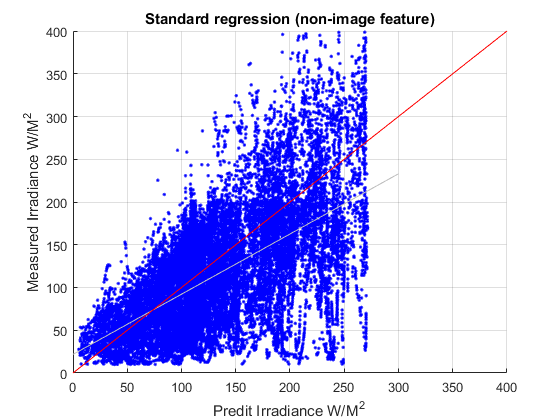
\includegraphics[scale=.6]{linear_regress_non_imag_new}
\centering
\end{figure}

In next step, we included all the features (non-image and image-based) for regression training. The feature selection algorithm only chose 12 features out of 27 features (i.e. $9+9+9$ for base features, square and square root). The selected features are indexes of [1 2 4 5 7 11 14 17 20 21 22 23] in the feature vector. This indicates that there is some non-linearity in the relation of features to targets. The result of linear regression on this feature vector shows an RMSE of 44.7  $W/m^2$ on the test data set and 47.4 for training set. The result for only using image-based features is always worse than non-image features by a distance of around 5\%. Thus, it is clear that there is a considerable improvement (26\%) in regression performance when using both non-image and image features. The reason for performing slightly better on test data can be indicating that Linear regression can't model this dataset well or there is a bias in errors of training. We also have tried a training set two times bigger than test set, but the same pattern was observed. The correlation of estimated DHI to target values is illustrated in Figure \ref{fig:ln_result_all}. 

\begin{figure}[h!]
\caption{Linear regression result using both feature types}
\label{fig:ln_result_all}
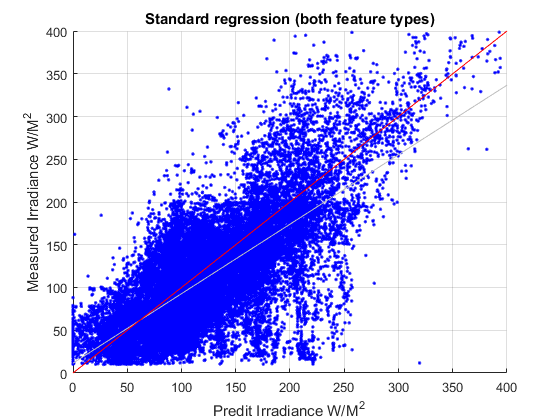
\includegraphics[scale=.6]{linear_regress_with_imag_new}
\centering
\end{figure}

To investigate distribution of errors, we have plotted the histogram of training and test errors for both non-image and full feature set in Figure \ref{fig:ln_result_hist}. One can see that error when using all the feature elements is clearly lower than when using only non-image features. Also, the training error is usually below the test error, but in the right edge of the plot the training error frequency exceeds the test error. This can indicate an underestimating bias in the training set which is due to relatively higher number of low-DHI samples in the data set.

\begin{figure}[h!]
\caption{Error histogram for linear regression}
\label{fig:ln_result_hist}
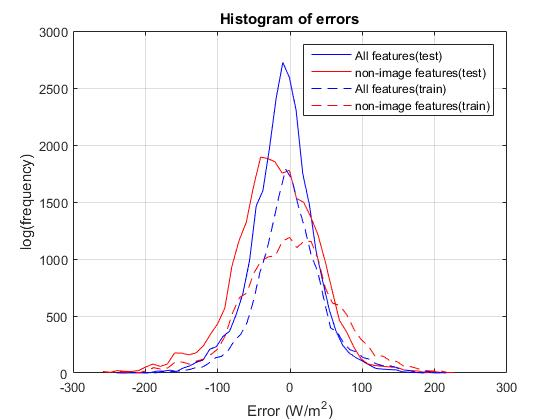
\includegraphics[scale=.8]{linear_regress_err_hist}
\centering
\end{figure}

%%%%%%%%%%%%%%%%%%%%%%%%%%%%%%%%%%%%%%%%%%
\section{K-NN regression}
For K-NN method, the non-image and full feature experiments is repeated as well. After trying different values of neighbors (K), K=10 showed the least error and is been used for the rest of experiments. For distance measure, we evaluated Manhattan distance and also $q=2$ (i.e. Euclidean) and $q=3$ for Minkowski. The results showed that Manhattan distance perform better for this application. This suggests that importance rank of features is very close to each other. The feature selection on non-image features only selects clear-sky-DHI and exclude sun-zenith due to its negligible importance. The table \ref{table:rmse_knn} displays the errors obtained using K-NN regression on training and test data. And the Figure \ref{fig:knn_result_no_image} shows correlation of results for non-image feature set.

\begin{table}[h!]
\centering
\begin{tabular}{ |p{2.5cm}||p{4cm}|p{4cm}|  }
%\hline
%\multicolumn{3}{|c|}{K-NN RMSE} \\
\hline
 &non-image features& both feature types\\
 \hline
 Training set &   58.2  & 35.7 \\
 Test set&   57.2  & \textbf{34.8} \\
 \hline
\end{tabular}
\caption{Regression errors of K-NN on non-image and full feature vectors}
\label{table:rmse_knn}
\end{table}

One can see that using both non-image and image-based features reduces RMSE by around 39\% from only using non-image based features.

\begin{figure}[h!]
\caption{K-NN estimation result using only non-image features}
\label{fig:knn_result_no_image}
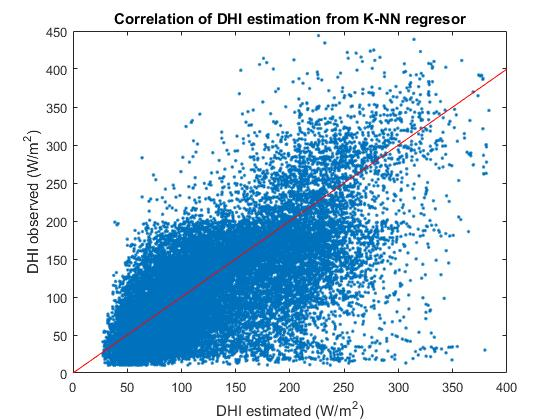
\includegraphics[scale=.6]{knn_result_no_image}
\centering
\end{figure}

Running the feature selection on base features for K-NN regressor results in leaving out the saturation factor feature. This indicates its negligible correlation to DHI which was not obvious at the time of creating feature list. This low importance can be due to the fact that for many images where sun is completely visible, the saturation factor (which is only defined for cloud pixels around sun) is trivially zero. And these images correspond to high DHI values while having zero saturation. However, there are many cloudy images where sun is not visible but because of think clouds, the saturation factor is again zero and DHI value is low. Therefore, we can see that the relation of DHI to saturation factor is more complex than linear or simple non-linear methods. Thus, deriving a more sophisticated feature from saturation factor, sun-state and circumsolar cloud coverage could be more relevant to diffuse irradiance. The correlation of K-NN result to DHI while using the selected features is depicted in Figure \ref{fig:knn_result_all} .

\begin{figure}[h!]
\caption{K-NN estimation result using all the features}
\label{fig:knn_result_all}
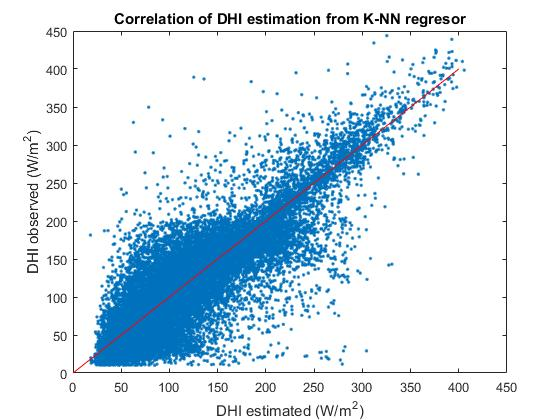
\includegraphics[scale=.6]{knn_result_with_image}
\centering
\end{figure}

The error histogram of result for K-NN method is illustrated in Figure \ref{fig:err_hist_knn}. This figure confirms that error when using both feature types is almost always below the error of non-image features alone. The training error is also below the test error except in the most right side of the plot where it goes above test error. The slightly higher training error in Table \ref{table:rmse_knn} can be related to this parts of the error histogram.

\begin{figure}[h!]
\caption{Error histogram for K-NN estimation result}
\label{fig:err_hist_knn}
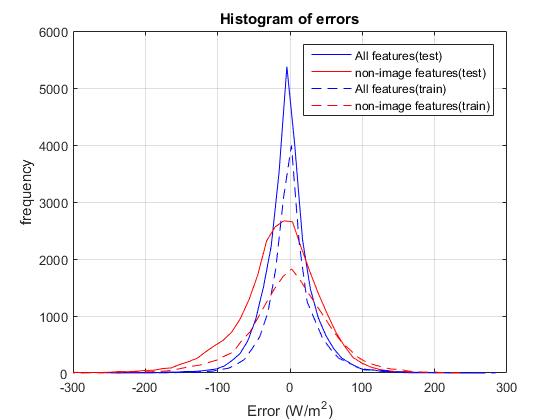
\includegraphics[scale=.7]{knn_result_error_hist}
\centering
\end{figure}

%%%%%%%%%%%%%%%%%%%%%%%%%%%%%%%%%%%%%%%
\section{SVR}
The performance of support vector regression is highly dependent on $C$, $\epsilon$ and $\gamma$ parameters which define trade off between model complexity (i.e. number of support vectors) and regression error and control influence of support vectors. Therefore, it is very important to tune these parameters on our specific dataset through k-fold cross validation. We are using 5-fold validation based on our training sample size. Thus, we randomly divide our training set into 5 equal sized partitions. Then for each parameter combination we use one of the folds for testing and the rest for training set. The final error of a parameter combination comes from averaging the errors for all the folds (5). After cross validation on possible ranges for $C$ and $\epsilon$  and $\gamma$ parameters, the best values are selected to be 250, 9 and 8 respectively. Besides RBF, linear and sigmoid kernels have been evaluated for this task, but RBF outperformed other kernel types and was selected for further experiments on SVR. The popular libsvm toolbox is used for training an SVM model and predicting DHI values. We have not applied feature selection directly on SVR due to its long runtime, however, we manually removed some feature elements such as saturation factor and circumsolar cloud coverage, and the error was decreased to 38.0. Therefore, we excluded them from features list for further experiments on SVR.\newline
The result of SVR is summarized in the table \ref{table:rmse_svr}. It shows an improvement of 38\% when using both non-image and image-based features. This can also be seen in Figures \ref{fig:svr_result_no_image} and \ref{fig:svr_result_all} which depicts correlation of SVR results to DHI values. Again, the vertical lines in Figure \ref{fig:svr_result_no_image} indicate a strong indifference of the learned model to cloud coverage conditions.

\begin{table}[h!]
\centering
\begin{tabular}{ |p{2.5cm}||p{4cm}|p{4cm}|  }
 %\hline
 %\multicolumn{3}{|c|}{SVR RMSE} \\
 \hline
 &non-image features& both feature types\\
 \hline
 Training set &   62.0  & 38.4 \\
 Test set&   62.7  & \textbf{38.0} \\
 \hline
\end{tabular}
\caption{Regression errors of SVR on non-image and both feature types}
\label{table:rmse_svr}
\end{table}

\begin{figure}[h!]
\caption{SVR result using only non-image features}
\label{fig:svr_result_no_image}
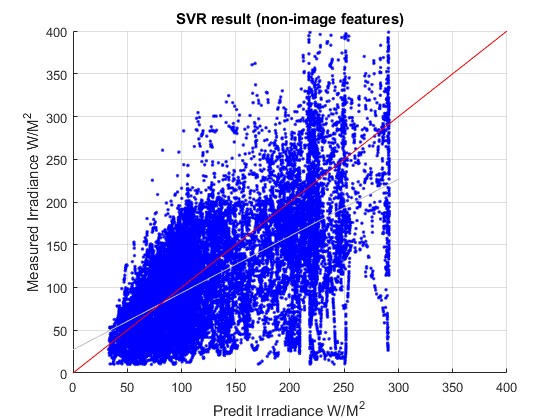
\includegraphics[scale=.6]{svr_result_no_image_new}
\centering
\end{figure}

\begin{figure}[h!]
\caption{SVR result using both feature types}
\label{fig:svr_result_all}
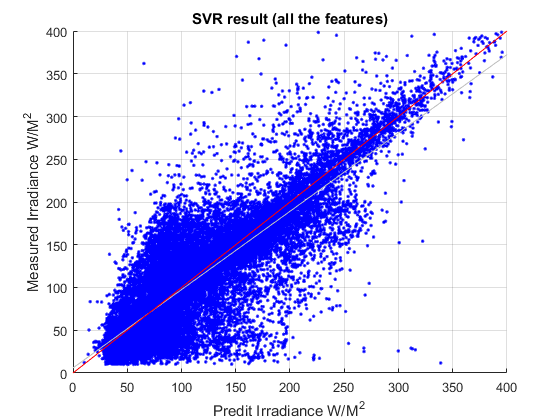
\includegraphics[scale=.6]{svr_result_all_features_new}
\centering
\end{figure}

The error histogram of error is plotted in Figure \ref{fig:err_hist_svr}. This shows more clearly the improvement of using image-based features. It also proves that the learned model from SVR method is relying on key features that are showing consistent behavior in training and test sets.

\begin{figure}[h!]
\caption{Error histogram for SVR result}
\label{fig:err_hist_svr}
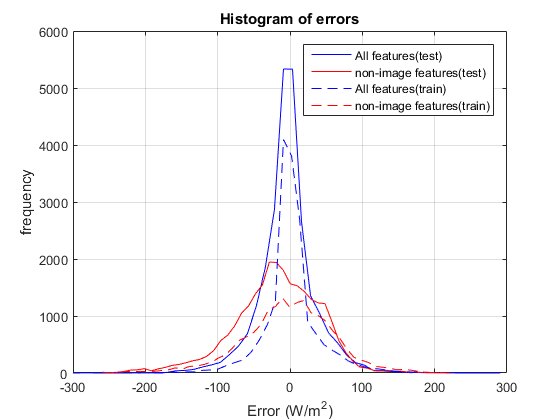
\includegraphics[scale=.7]{svr_error_histogram_new}
\centering
\end{figure}

%%%%%%%%%%%%%%%%%%%%%%%%%%%%%%%%%%%%%%%%%%
\section{Some error cases}
As we see in the error histograms, the range of error values in all regression method is considerable and between -200 to 200 $W/m^2$. However, the number of these high value errors are very small and can be seen as outliers in statistical analysis.  After looking at the corresponding images and their feature vectors we realized that the reason for such abnormal regression result is either failure in cloud segmentation algorithm or misclassifying sun-state. For example, Figure \ref{fig:img_fail1} shows an image where the predicted DHI is around 300$W/m^2$ but observed value is around 20. The reason for this off prediction is the rain drops on the camera which prevented the cloud in circumsolar area to be detected. Therefore, the K-NN matches this image to other images with clear area around the sun and consequently results in high DHI prediction. Handling rain drops in images is challenging task which is out of the scope of this thesis.

\begin{figure}[h!]
\caption{An image sample of large estimation error}
\label{fig:img_fail1}
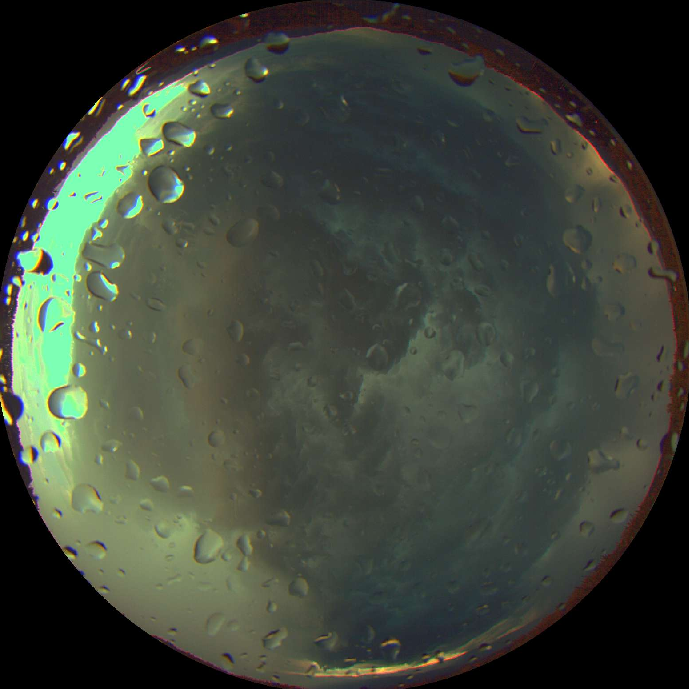
\includegraphics[scale=.4]{fail1}
\centering
\end{figure}


Another bad prediction is displayed in Figure \ref{fig:img_fail2} where sun-state is detected as 1 which means sun is not visible at all in the image, but we can clearly see the sun passing the light through a thin cloud. However, the saturation factor is been calculated correctly for this image. The reason for misclassifying sun-state is that the sun detection algorithm looks for a big enough black dot in circumsolar area that is surrounded with bright pixels up to a specific radius. But the black dot of sun in this image is not big enough to be detected by that algorithm. By adjusting the threshold, this case can be correctly classified, but some other false positive instances might appear in other images.

\begin{figure}[h!]
\caption{An image sample of large estimation error}
\label{fig:img_fail2}
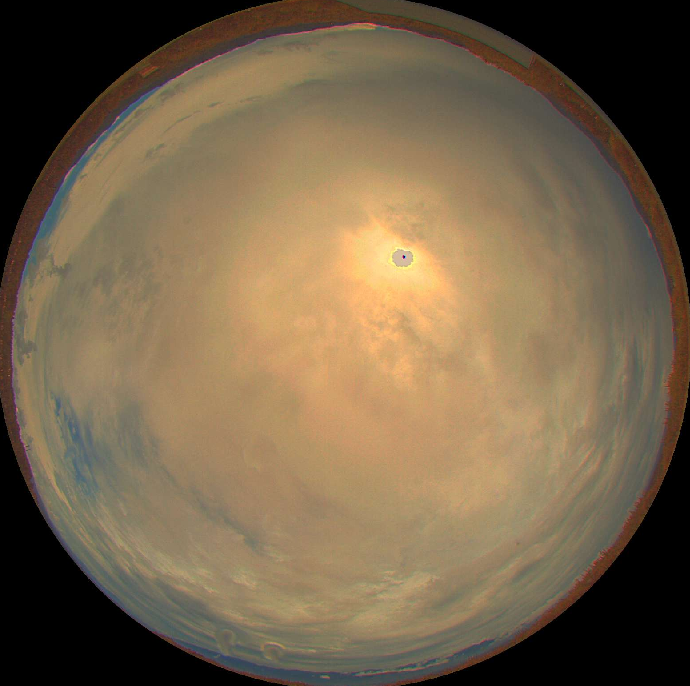
\includegraphics[scale=.4]{fail2}
\centering
\end{figure}

Again in another false prediction case, Figure \ref{fig:img_fail3} shows an image with strange colors in the horizon and clouds. Therefore, cloud segmentation failed to detect those clouds and reported 3\% cloud coverage, thus predicting a high DHI while the actual value is around 17.

\begin{figure}[h!]
\caption{An image sample of large estimation error}
\label{fig:img_fail3}
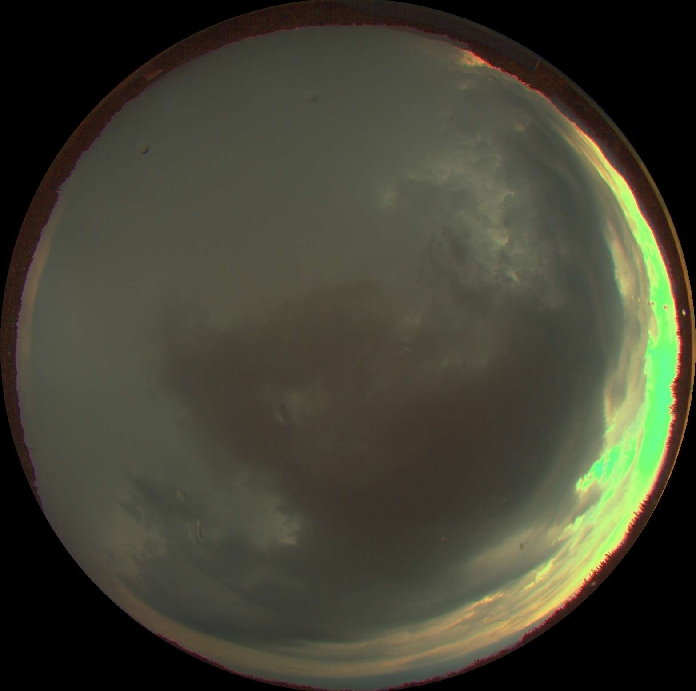
\includegraphics[scale=.4]{fail3}
\centering
\end{figure}

\section{Comparison}
As we saw before, using image-based features along non-image features improves the regression accuracy considerably. Now, for choosing the best performing method among the three regression algorithms, we compare the RMSE of their result for the case where both feature types were used. As Table \ref{table:rmse_cmp} clarifies, K-NN method outperforms linear regression by 20\% and support vector regression by around 9\% improvement.

\begin{table}[h!]
\centering
\begin{tabular}{ |p{2cm}||p{4cm}|p{2cm}|p{2cm}|  }
 %\hline
 %\multicolumn{4}{|c|}{RMSE full feature list} \\
\hline
 &Linear Regression& K-NN & SVR\\
 \hline
Test error& 44.7 & \textbf{34.8} & 38.0\\
 \hline
\end{tabular}
\caption{Comparison of RMSE for all three regression methods using both feature types}
\label{table:rmse_cmp}
\end{table}

However, bigger training set can reduce these errors. It's specifically more beneficial for K-NN since it relies on finding similar cases in training data for every test instance. On the other hand, by using other kernel types or a better feature selection, we might be able to improve the performance of SVR, but it's not guaranteed. Therefore, we choose \textbf{K-nearest-neighbor} with full feature list as the best method for DHI prediction for our application which achieves around 40\% improvement compared to using only non-image features. Since no other work exists with similar experimental setup and clear algorithm, we could not compare result of our method to other recent research in this area.

